% !TEX root = report.tex

% Основной стиль текста на странице

\documentclass[a4paper, oneside, 14pt, final]{extreport}

% \usepackage[T2A]{fontenc}
% \usepackage[utf8]{inputenc}
\usepackage[english, russian]{babel}

\usepackage{fontspec}
\setmainfont{Times New Roman}

\usepackage[top=20mm, bottom=27mm, left=30mm, right=15mm]{geometry}

\linespread{1.15} % Recommended: 1.00, 1.15, 1.25

\newlength{\parinlen}
\setlength{\parinlen}{12.5mm} % Recommended: 1.25cm, 1.27cm

\usepackage{indentfirst}
\setlength{\parindent}{\parinlen}    

% Стиль сносок

\usepackage{perpage}
\MakePerPage{footnote}

\makeatletter 
    \def\@makefnmark{\hbox{\@textsuperscript{\normalfont\@thefnmark)}}}
\makeatother

\usepackage[bottom]{footmisc}

% Стиль содержания

\usepackage{tocloft}

\setlength{\cftbeforetoctitleskip}{-1em}
\setlength{\cftaftertoctitleskip}{1em}

\makeatletter
\renewcommand{\cftsecfillnum}[1]
{%
    \ifnum#1<10%
    \gdef\@pnumwidth{6pt}%
    \else%
    \ifnum#1<100%
    \gdef\@pnumwidth{14pt}%
    \else%
    \gdef\@pnumwidth{18pt}%
    \fi\fi%
    {\cftsecleader}\nobreak%
    \makebox[\@pnumwidth][\cftpnumalign]{\cftsecpagefont #1}\cftsecafterpnum\par%
}

\renewcommand{\cftsubsecfillnum}[1]
{%
    \ifnum#1<10%
    \gdef\@pnumwidth{6pt}%
    \else%
    \ifnum#1<100%
    \gdef\@pnumwidth{14pt}%
    \else%
    \gdef\@pnumwidth{18pt}%
    \fi\fi%
    {\cftsecleader}\nobreak%
    \makebox[\@pnumwidth][\cftpnumalign]{\cftsubsecpagefont #1}\cftsubsecafterpnum\par%
}
\makeatother

\renewcommand{\cftsecleader}{\cftdotfill{\cftsecdotsep}}
\renewcommand{\cftsubsecleader}{\cftdotfill{\cftsubsecdotsep}}

\renewcommand\cftsecdotsep{\cftdot}
\renewcommand\cftsubsecdotsep{\cftdot}

\cftsetindents{section}{0.5em}{1.0em}
\cftsetindents{subsection}{1.5em}{1.8em}

% Стиль колонтитулов

\usepackage{fancyhdr} 
\pagestyle{fancy}

\fancyhf{}
\fancyfoot[R]{\thepage} 

\renewcommand{\footrulewidth}{0pt}
\renewcommand{\headrulewidth}{0pt}

\fancypagestyle{plain}{\fancyhf{}\rfoot{\thepage}}

% Стиль секций

\setcounter{secnumdepth}{3}

\renewcommand{\thesection}{\arabic{section}}

\makeatletter
\renewcommand{\@seccntformat}[1]{\csname the#1\endcsname{}~}

\renewcommand{\section}
{%
    \clearpage%
    \@startsection{section}{1}%
    {\parinlen}%
    {-1em \@plus -1ex \@minus -.2ex}%
    {1em \@plus .2ex}%  
    {\raggedright\normalfont\normalsize\bfseries\MakeUppercase}%
}

\renewcommand{\subsection}
{%
    \@startsection{subsection}{2}%
    {\parinlen}%
    {-1em \@plus -1ex \@minus -.2ex}%
    {1em \@plus .2ex}% 
    {\raggedright\normalfont\normalsize\bfseries}%
}

\renewcommand{\subsubsection}
{%
    \@startsection{subsubsection}{3}%
    {\parinlen}%
    {-1em \@plus -1ex \@minus -.2ex}%
    {1em \@plus .2ex}%                         
    {\raggedright\normalfont\normalsize\bfseries}%
}

\newcommand{\@csection}
{%
    \clearpage%
    \@startsection{section}{1}%
    {\z@}%                                   
    {-1em \@plus -1ex \@minus -.2ex}%
    {1em \@plus .2ex}%
    {\centering\normalfont\normalsize\bfseries}%
}

\newcommand{\csection}[1]
{%
    \@csection*{\MakeUppercase{#1}}%
    \addcontentsline{toc}{section}{#1}%
} 

\newcounter{appendix}
\renewcommand{\theappendix}{\Asbuk{appendix}}

\newcommand{\@appendix}
{%
    \clearpage%
    \@startsection{section}{1}%
    {\z@}%                                   
    {-1em \@plus -1ex \@minus -.2ex}%
    {1em \@plus .2ex}%
    {\centering\normalfont\normalsize\bfseries}%
}

\renewcommand{\appendix}[2]
{%
    \refstepcounter{appendix}%
    \@appendix*{\MakeUppercase{Приложение \theappendix} \\ (#1) \\ #2}%
    \markboth{\MakeUppercase{#1}}{}%
    \addcontentsline{toc}{section}{Приложение {\theappendix} (#1) #2}%
}
\makeatother

% Графические изображения

\usepackage[final]{graphicx}
\DeclareGraphicsExtensions{.pdf,.png,.jpg,.eps}
\graphicspath{{images/}}

% Позиционируемые графические изображения

\usepackage{float}

% Стиль надписей к таблицам и изображениям

\usepackage[nooneline]{caption}
\usepackage{subcaption}

\DeclareCaptionLabelSeparator{stb}{~--~}

\DeclareCaptionLabelFormat{stbfigure}{Рисунок #2}
\DeclareCaptionLabelFormat{stbtable}{Таблица #2}

\captionsetup[figure]{labelformat=stbfigure, justification=centering, labelsep=stb, size=normalsize}
\captionsetup[table]{labelformat=stbtable, justification=raggedright, labelsep=stb, size=normalsize}

% Математика и оформление формул

\usepackage{calc}
\usepackage{amsmath}
\usepackage{amsfonts}
\usepackage{amssymb}
\usepackage{amsthm}

% \newlength{\eqindent}
% \setlength{\eqindent}{1.4em} % Recommended: baselineskip, 1.3em, 1.4em, 1.5em

% \makeatletter
% \expandafter\def\expandafter\normalsize\expandafter
% {%
%     \normalsize
%     \setlength\abovedisplayskip{\eqindent - \baselineskip}
%     \setlength\belowdisplayskip{\eqindent}
%     \setlength\abovedisplayshortskip{\eqindent - \baselineskip}
%     \setlength\belowdisplayshortskip{\eqindent}
% }
% \makeatother

\newenvironment{explanation}
{\begin{itemize}[leftmargin=0cm, itemindent=\widthof{где} + \labelsep , labelsep=\labelsep]\renewcommand{\labelitemi}{}}
{\end{itemize}}

% Нумерация и стиль перечислений

\usepackage{enumitem}

\makeatletter
    \AddEnumerateCounter{\asbuk}{\@asbuk}{щ)}
\makeatother

\setlist{nolistsep}

\renewcommand{\labelenumi}{\arabic{enumi}}

\setlist[itemize,0]{itemindent=\parindent + 2.2ex, leftmargin=0ex, label=--}
\setlist[enumerate,1]{itemindent=\parindent + 2.7ex, leftmargin=0ex}
\setlist[enumerate,2]{itemindent=\parindent + \parindent - 2.7ex}

\AtBeginDocument{\numberwithin{equation}{section}}
\AtBeginDocument{\numberwithin{table}{section}}
\AtBeginDocument{\numberwithin{figure}{section}}

% Вспомогательные пакеты

\usepackage{makecell}
\usepackage{multirow}
\usepackage{array}
\usepackage{longtable}
\usepackage{pdfpages}
\usepackage{textcomp, gensymb}
\usepackage{tabularx}

% Стиль библиографии

\usepackage[square, numbers, sort&compress]{natbib}

\setlength{\bibsep}{0em}

\bibliographystyle{gost780u}

\setlength\bibindent{-1.0900cm}

\makeatletter
\renewcommand\NAT@bibsetnum[1]
{%
    \settowidth\labelwidth{\@biblabel{#1}}
    \setlength{\leftmargin}{\bibindent}\addtolength{\leftmargin}{\dimexpr\labelwidth+\labelsep\relax}%
    \setlength{\itemindent}{-\bibindent+\parinlen-0.240cm}%
    \setlength{\listparindent}{\itemindent}%
    \setlength{\itemsep}{\bibsep}\setlength{\parsep}{\z@}%
    
    \ifNAT@openbib
        \addtolength{\leftmargin}{\bibindent}%
        \setlength{\itemindent}{-\bibindent}%
        \setlength{\listparindent}{\itemindent}%
        \setlength{\parsep}{10pt}%
    \fi
}
\makeatother

% Поддержка ссылок с нижним подчеркиванием в BibTeX

\usepackage{url}
\urlstyle{same}

\def\UrlBreaks{\do\/\do-}

% Frenchspacing и перенос слов с дефисом

\def\hyph{-\penalty0\hskip0pt\relax}

\frenchspacing

% Гиперссылки в содержании и тексте

\usepackage[colorlinks=true, allcolors=black]{hyperref}

% Листинги кода

\usepackage{fancyvrb}
\usepackage{verbatim}

\usepackage{fancyvrb} % внести в следующую версию преамбулы
\usepackage{verbatim}

\begin{document}

    \thispagestyle{empty}

\begin{center}
  Министерство образования Республики Беларусь\\[1em]
  Учреждение образования\\
  БЕЛОРУССКИЙ ГОСУДАРСТВЕННЫЙ УНИВЕРСИТЕТ\\
  ИНФОРМАТИКИ И РАДИОЭЛЕКТРОНИКИ\\[2em]

  \begin{minipage}{\textwidth}
    \begin{flushleft}
      Факультет компьютерных систем и сетей\\[1em]
      Кафедра электронных вычислительных машин\\[1em]
    \end{flushleft}
  \end{minipage}\\[1em]

  \vspace{3em}
  \hfill 
  \textit{\MakeUppercase{К защите допустить}}\\
  \vspace{0.6em}
  \hfill 
  \underline{\hspace{2.7cm}}\textit{~Л.~П.~Поденок} % todo: make transform

  \vfill
    ПОЯСНИТЕЛЬНАЯ ЗАПИСКА \\
    к курсовому проекту \\
    на тему \\
    \MakeUppercase{Драйвер USB клавиатуры} \\ 
    БГУИР КП 1-40 02 01 310 ПЗ \\

  \vfill

  \begin{tabular}{p{0.30\textwidth}p{0.30\textwidth}p{0.30\textwidth}}
    Студент гр.~150503     &&   А.~В.~Кутняк  \\
                           &&                 \\
    Руководитель           &&   Д.~В.~Басак   \\
  \end{tabular}
  
  \vfill

  {\normalsize Минск \the\year}
\end{center}

\pagebreak % не знаю, почему, но vfill не заполняет всю страницу                   % Титульный лист пояснительной записки
    
\includepdf[pages={1}, pagecommand={\thispagestyle{empty}}]{resources/Tech.pdf}                    % Техническое задание проекта
    \renewcommand\contentsname{\centerline{\bfseries\normalsize{\MakeUppercase{содержание}}}}
{
    \normalsize\selectfont
    \tableofcontents
    \newpage
}                     % Содержание пояснительной записки
    
    \csection{Введение}

% Учебная практика является обязательным элементом подготовки специалиста с высшим 
% образованием и одной из форм текущей аттестации студента по учебной дисциплине. 
% Для студентов это первая учебная работа такого рода и объёма. 
% Реферат содержит результаты теоретического исследования по теме «Концепция Интернет вещей (IoT)», что способствует получению базовых навыков по поиску и систематизации информации, а также подготовке к дальнейшему изучению технологий, которые относятся к концепции IoT.


% В первом разделе дается базовая информация о концепции интернета вещей, 
% а также возможные области применения. 
% Описываются задачи, которые помогает решать данная область, возможные способы реализации.


% Второй раздел описывает основные характеристики технологии IoT, 
% методы использования устройств, которые можно отнести к заданной концепции, 
% а также части, без которых концепцию невозможно будет реализовать. 
% Третий раздел информирует о преимуществах технологии, а так же о недостатках. 


% Четвертый и пятый разделы описывают возможные реализации устройств экосистемы IoT,
% а также используемое программное обеспечение, 
% которое заложено в реализацию концепции IoT.


% Раздел шесть и семь содержат информацию об используемых протоколах передачи информации 
% между устройствами в сети, а так же более подробно описывают аспекты безопасности 
% системы интернета вещей.

Учебная ознакомительная практика является неотъемлемой частью образовательного 
процесса в высших учебных заведениях.

Целью ознакомительной практики является выработка профессиональных навыков
в поиске и обработке информации, а также её обработки и представлении
в соотвествии с указанными требованиями и стандартами.

Данный реферат содержит результаты теоретического исследования по теме
<<Методы машинного обучения в системах обработки звуковых и речевых сигналов>>,
которая является одним из перспективных направлений для решения 
существующих практических задач.

В первом разделе содержатся базовые понятия из области машинного обучения.
Дается представление о задаче обучения по прецендентам, перечисляются основные преимущества
методов машинного обучения перед вычислительными методами, а также перечисляются классические задачи машинного 
обучения и способы машинного обучения, используемые при решении данных задач.

Во втором разделе представлен материал по представлению звуковых сигналов для их обработки
в системах, использующих методы машинного обучения.

В третьем разделе дается представление о методах машинного обучения,
применяемых в обработке звуковых и речевых сигналов. 
Описывается архитектура нейронных сетей прямого распространения, а также классический метод их обучения.
Рассматривается архитектура сверточных нейронных сетей, принцип их действия,
основные преимущества их использования.

Четвертый раздел посвящен одной из основных задач обработки звуковых сигналов -- шумоподавлению.
В разделе содержится постановка задачи шумоподавления, а также примеры некоторых
нейросетевых архитектур, используемых для решения данной задачи.    % Введение

    \section{Теоретические сведения}

Для понимания того, как реализовать свой язык программирования,
необходимо понимать, что такое \emph{язык программирования}.

Данный раздел содержит краткие сведения о языках программирования,
а также об их сходствах и различиях.

%\subsection{Понятие языка программирования}
\subsection{Основные понятия из теории языков программирования}

\emph{Язык программирования} -- это формальный язык,
который может использоваться для записи компьютерных программ.

В информатике под \emph{формальным языком} понимают некоторое
множество конечных слов над конечным алфавитом.

Язык программирования определяет набор 
\emph{лексических}, \emph{синтаксических} и \emph{семантических} 
правил, которые определяют внешний вид программы, а также действия, 
которые она будет исполнять.

\emph{Лексика} определяет множество слов языка, т.е. то,
как из алфавита языка образуются определенные слова.

\emph{Синтаксис} определяет набор правил, по которым
описываются комбинации слов языка,
считающихся правильно структурированными программами.

\emph{Семантика} определяет набор правил, которые 
придают смысл синтаксически правильным программам.

Итак, язык программирования -- это совокупность правил,
определяющих структуру программы, слов, из которых она состоит,
а также то, что на основании этой программы будет выполнять
некоторая исполнительная машина.

Помимо основных правил, на которых строится язык,
существует множество специальных терминов, дающих ему
некоторую условную характеристику, 
например, \emph{динамическая типизация}, 
или \emph{явное преобразование типов}, однако все они
не входят в тему данной работы. Более важным для нас являются 
не столько термины из области \emph{стандартизации} 
языков программирования, сколько
термины и определения из области их \emph{реализации}.

%\subsection{Понятие транслятора}

Наиболее распространенной классификацией реализаций языков
программирования по типу исполнения является
разделение языков на \emph{интерпретируемые} и \emph{компилируемые}.

Интерпретаторы и компиляторы, ответственные за соответствующие
им процессы \emph{интерпретации} и \emph{компиляции},
относятся к одному более общему классу программ -- \emph{трансляторам}.

\emph{Транслятор} -- это техническое средство, выполняющее трансляцию,
т.е. преобразование исходной программы на одном из языков программирования,
в программу, написанную на другом языке.

Суть операции трансляции заключается в том, что программа на неизвестном
для исполнительной машины языке переводится в понятнее для нее представление,
после чего становится возможным исполнение на этой машине исходной программы.

\emph{Компиляция} -- это техника выполнения, при которой 
исходный код программы на исходном языке транслируется,
обычно, в программу на языке более низкого уровня.

Когда мы говорим, что программа является \emph{компилятором},
мы подразумеваем что она переводит программу в какое-то
другое представление, но не исполняет ее. 
Пользователь получает результат \emph{компиляции}
и исполняет его самостоятельно, используя имеющиеся у него
для этого инструменты.

Когда же мы говорим, что программа является \emph{интерпретатором},
мы имеем ввиду то, что она получает на вход исходный код программы
и немедленно приступает к его исполнению, то есть 
запускает программу "из исходников".

Однако исполнение программы "из исходников" не означает,
что интерпретатор не преобразует, то есть не \emph{транслирует}
исходный код программы в иное представление.

В качестве примера можно рассмотреть основную реализацию языка
Python - интерпретатор CPython.
С точки зрения пользователя CPython действительно является
интерпретатором: он принимает на вход программу и сразу же
приступает к ее исполнению.
Однако с точки зрения технической реализации CPython содержит
в себе множество деталей, присущих компиляторам.

Он разбирает исходную программу и преобразует ее в древовидную
структуру (AST - Abstract Syntax Tree),
затем анализирует полученное представление и транслирует его 
в более простое промежуточное (IR - Intermediate Representation),
роль которого выполняет байткод,
после чего исполняет полученный байткод посредством JIT-компиляции.

В книге Роберта Нистрема <<Создание интерпретаторов>> вопрос
о разнице между интерпретаторами и компиляторами сравнивается
с вопросом о разнице между фруктами и овощами.
Несмотря на то, что выбор между фруктами и овощами выглядит
как взаимоисключающий, слово \emph{фрукт} является ботаническим
термином, а слово \emph{овощ} -- термином из кулинарии.
Таким образом всегда найдется овощ, который не является фруктом,
например, \emph{морковь}, но это вовсе не означает, что не найдется 
съедобного растения, являющегося и фруктом, и овощем, 
например \emph{томата}.

%\subsection{Краткие сведения об языке Basic}
\subsection{Краткие сведения об языке Бейсик}

Бейсик (BASIC, 
сокращение от англ. Beginner's All-purpose Symbolic Instruction Code 
-- универсальный код символических инструкций для начинающих) 
-- название семества языков высокого уровня.

Был разработан в 1964 году как инструмент,
при помощи которого студенты-непрограммисты
имели бы возможность создавать компьютерные программы для решения
собственных задач. 

Получил широкое распространение в качестве 
\emph{языка для домашнего компьютера}.

Внешний вид программ написанных на ранних версиях Бейсика
во многом определялся тем, что он предназначался для 
среды программирования со строковым редактором текста.
В таком редакторе пользователь не имел возможности отображать
весь текст на экране, а также перемещаться по нему в любых
направлениях с помощью перефирийных устройств.
В строковых редакторов для редактирования строки текста
пользователь должен был дать команду изменения строки с заданным
номером, а затем ввести новый текст указанной строки.
Для вставки новой строки нужно было дать команду вставки,
указав правильный номер.
Вводимые таким образом строки можно было отобразить на экране
согласно их нумерации при помощи специальной команды \emph{List}.

%\subsection{Описание синтаксиса языка Бейсик} % ???

Как уже было сказано ранее, на синтакис Бейсика главным образом 
повлияла среда программирования, на которой он использовался.

Ранние версии языка содержали очень малое число ключевых слов:
их количество могло не достигать и 20.

Программа языка была представлена набором строк,
пронумерованных целыми числами, называемыми метками строк.

Далее строка содержала инструкцию языка, которая завершалась 
символом перехода на новую строку. Существовали реализации,
которые позволяли помещать несколько инструкций на одной строке,
разделяя их символом двоеточия <<:>>.

Ниже представлен список основных инструкций:

\begin{itemize}
    \item <<Input ["Приглашение"], Переменная>> -- вывод на экран
          опционального приглашения на ввод и чтение
          значения с клавиатуры в переменную.
          
    \item <<Print 
          (\emph{Текст} | \emph{Переменная}) 
          ; ... ; 
          (\emph{Текст} | \emph{Переменная})>> --
          вывод перечисляемых значений на экран.

    \item <<Let \emph{Переменная} = \emph{Значение}>> -- операция 
          присваивания значения переменной, 
          ключевое слово Let в большинстве реализаций
          предполагалось как опциональное.

    \item <<Goto \emph{Метка}>> -- безусловный переход на строковую метку.
    
    \item <<If \emph{Условие} Then ...> -- условный оператор.
    
    \item <<While \emph{Условие}>> -- заголовок цикла с условием.
    
    \item <<Endw> -- завершение тела цикла.
    
    \item <<For \emph{Переменная} = \emph{Начало} 
          To \emph{Конец} [Step \emph{Шаг}]>> -- заголовок
          цикла с шагом, параметр Step являлся опциональным и 
          в случае его отсутствия шаг цикла равнялся 1.
\end{itemize}

В реализациях языка с интерактивным режимом поддерживались
команды, необходимые для взаимодействия исполняемой
среды с пользовательским терминалом, а также команды взаимодействия
с файловой системой и перефирийными устройствами.

Также ранние реализации языка содержали специфические ограничения:
длина идентификатора переменной не превышала одного символа,
а типизация обеспечивалась специальными суффиксами
('\$' для строковых типов, '\%' для целочисленных и т.д.).       % Теоретические сведения
    \section{Представление звукового сигнала}

\subsection{Дискретизация звукового сигнала}

Для обработки в машине данные должны быть представлены в цифровом виде.
В то время как текстовая и графическая информация представляется
непосредственным двоичным кодированием наименьшей единицы информации
(символ в тексте и пиксель в изображении), аналоговый звуковой сигнал
представляет собой механическую волну.

Так как звуковая волна может быть описана как функция её амплитуды от времени,
для представления звукового сигнала в цифровом виде можно применить
его дискретизацию.

В математике под дискретизацией понимают представление непрерывной функции
дискретной совокупностью её значений при различных наборах аргументов.

Временная дискретизация звука -- процесс кодирования непрерывного звукового сигнала,
при котором волна разбивается на отдельные небольшие интервалы, для каждого из которых
устанавливается определенное значение амплитуды звуковой волны. 
Амплитуда показывает, насколько громкий звук на данном участке.

На рисунке \ref{fig:section2:discrete} изображен пример
дискретизации аналогового звукового сигнала.

\begin{figure}[h!]
    \centering
    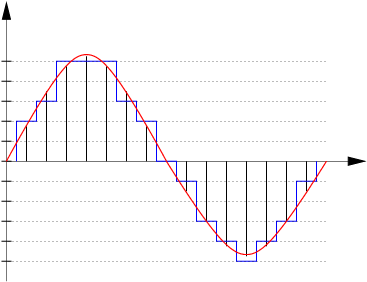
\includegraphics[scale=1]{S2IM1.png}
    \caption{Пример дискретизации звукового сигнала}
    \label{fig:section2:discrete}
\end{figure}

\subsection{Представление сигнала в виде спектрограммы}

Для использования методов машинного обучения в обработке звуковых и речевых сигналов
для получения более подробной информации о звуке, а также для более простого представления
звукового сигнала, звук представляют графически в виде спектрограмм.

Для введения понятия спектрограммы определим понятие спектральной плотности мощности звукового сигнала.

\emph{Спектральной плотностью мощности} в физике и теории обработки сигналов называется функция,
описывающая распределение мощности сигнала в зависимости от его частоты \cite{goldenberg}. 

Спектрограмма -- это изображение, которое показывает зависимость спектральной плотности мощности сигнала от времени.

Наиболее распространенным видом спектрограммы является двумерная диаграмма, по горизонтальной оси которой идет отсчет времени,
а по вертикальной -- отсчет частоты. Третье измерение спектрограммы, указывающее амплитуду, 
представляется интенсивностью или цветом каждой точки плоскости изображения.

\begin{figure}[h!]
    \centering
    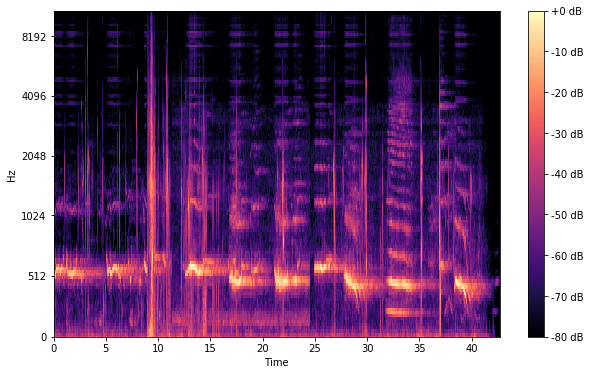
\includegraphics[scale=0.6]{S2IM2.png}
    \caption{Пример спектрограммы звукового сигнала}
\end{figure}

Получить спектрограмму звукового сигнала можно используя метод быстрого оконного преобразования Фурье,
который генерирует спектры за счет разделения исходного звукового сигнала на интервалы методом скользящего окна.       % Постановка задачи
    \section{Структура входных и выходных данных}

\subsection{Входные данные}

Входные данные представлены текстовым файлом с исходным текстом программы на языке Бейсик.

Синтаксис данной реализации языка можно определить в виде расширенной формы Бэкуса-Наура
следующего вида:

\begin{Verbatim}[fontsize=\small]
    CHARS = ? все допустимые символы ?
    EOL   = ? символ окончания строки ?
    EOF   = ? символ окончания файла ?

    DIGIT = '0' | '1' | '2' | '3' | '4' | 
            '5' | '6' | '7' | '8' | '9'
    ALPHA = 'A' | 'B' | 'C' | 'D' | 'E' | 'F' | 'G' | 'H' | 
            'I' | 'J' | 'K' | 'L' | 'O' | 'M' | 'N' | 'P' | 
            'Q' | 'R' | 'S' | 'T' | 'U' | 'V' | 'W' | 'X' | 
            'Y' | 'Z'

    IDENTIFIER = (ALPHA) {ALPHA | DIGIT}
    INTEGER    = (DIGIT) {DIGIT}
    FLOATING   = (INTEGER) ['.'  INTEGER]
    STRING     = '"' {CHARS} '"' 

    PROGRAM  = COMPOUND
    COMPOUND = {LINE}
    LINE     = STATEMENT EOL
    
    STATEMENT = IF | FOR | WHILE | ASSIGN | INPUT | PRINT

    IF     = 'IF' BEXPR 'THEN' (LIF | MIF)
    LIF    = STATEMENT
    MIF    = EOL BEXPR ['ELSE' COMPOUND] 'ENDIF'

    FOR    = 'FOR' IDENT '=' NEXPR 'TO' NEXPR COMPOUND 'NEXT'
    WHILE  = 'WHILE' BEXPR COMPOUND 'WEND'

    ASSIGN = IDENT '=' NEXPR
    
    INPUT [STRING], IDENT
    PRINT (EXPR) {';' EXPR}
    
    SEXPR = ? строчные выражения ?
    NEXPR = ? числовные выражения ?
    BEXPR = ? логические выражения ?
\end{Verbatim}

Выражения в языке строятся согласно семантическим правилам операций,
перечисленных ниже:
\begin{itemize}
    \item Бинарные арифметические операции над числами.

    \item Бинарные операции логического сложения и умножения.

    \item Бинарные операции сравнения чисел.
    
    \item Унарные операции 'плюс' и 'минус' для чисел.

    \item Унарная операция логического отрицания.
    
    \item Числовые, логические, строковые терминалы.
    
    \item Скобочная вложенность.
\end{itemize}

\subsection{Выходные данные}

Выходными данными интерпретатора можно считать
результат выполнения операций \emph{Input} и \emph{Print},
возможные сообщения об ошибках,
а также внутреннее состояние памяти, отвечающей за хранение
переменных программы.       % Структура входных и выходных данных
    \section{Разработка программных модулей}

Как уже было отмечено в разделе \ref{system-design},
архитектура драйвера, реализованного в рамках данной работы,
не предполагает модульной архитектуры, а потому в качестве модулей
рассматриваются группы функций, выполняющих схожие задачи.

\subsection{Разработка группы вспомогательных функций}

В подразделе \ref{utility-group-design} упоминалось, что функции из данной
группы отвечают за выделение и освобождение памяти полей структуры \texttt{usbkeyboard},
поэтому, для дальнейшего обсуждения их реализации, необходимо привести ее определение:
\begin{verbatim}
struct usbkeyboard {
    struct input_dev* dev;
    struct usb_device* usbdev;

    struct urb* irq;
    struct urb* led;

    struct usb_ctrlrequest* creq;

    char name[KBD_NAME_MAX];
    char phys[KBD_PHYS_MAX];

    unsigned char prev_presses[8];
    unsigned char* presses;

    unsigned char curr_leds;
    unsigned char* leds;    

    dma_addr_t presses_dma;
    dma_addr_t leds_dma;

    bool leds_urb_submitted;
    spinlock_t leds_lock;
};
\end{verbatim}

Поля \texttt{dev} и \texttt{usbdev} выполняют указание на системные структуры
устройства ввода и устройства последовательной шины.

В свою очередь \texttt{irq} и \texttt{led} указывают на URB, первый из которых
отвечает за получение состояния нажатия клавиш, 
а второй -- за установку состояния светодиодов.

Символические массивы \texttt{name} и \texttt{phys} хранят название устройства
и его физический путь (в представлении топологии шины).

Массив \texttt{prev\_presses} хранит предыдущее состояние нажатий,
а указатель \texttt{presses} ссылается на память, используемую для хранения
получаемого от устройства состояния нажатий.

Поля \texttt{curr\_leds} и \texttt{leds} имеют назначение, аналогичное
предыдущим, за тем лишь исключением, что размер переменной предыдущего состояния
и размер памяти текущего состояния составляет один байт, что соответствует 
сведениям, представленным в таблице \ref{leds}.

Самыми интересными с точки зрения взаимодействия с памятью являются
поля \texttt{presses\_dma} и \texttt{leds\_dma}.
Данные поля хранят адрес прямого доступа к памяти (DMA),
механизм которого используется для совместного доступа к памяти
как со стороны процессора, так и со стороны самого устройства.
Выделение памяти для \texttt{presses} и \texttt{leds} осуществляется
при помощи функции \texttt{usb\_alloc\_coherent}
\footnote{
    coherent, когерентный, в данном контексте означает
    <<согласованный>>, предоставляющий совместный доступ.
},
одним из аргументов которой является \texttt{dma\_addr\_t*}.
В результате вызова функции возвращается указатель на буфер в CPU-пространства,
согласованный с DMA, а по адресу \texttt{dma\_addr\_t*} возвращается DMA-адрес буфера.
Чаще всего данный подход используется для того,
чтобы устройство на шине могло записывать данные в оперативную память
напрямую, не прерывая вычисления процессора.
Подробнее о технологии прямого доступа к памяти,
а также о предоставляемых операционной системой Linux возможностях, 
можно прочитать в источниках \cite{dma, ldd3}.

Поле \texttt{creq} содержит в себе структуру управляющего
запроса, используемого для отправки запроса на изменение состояния светодиодов 
устройства клавиатуры.

Оставшиеся поля \texttt{leds\_usb\_submitted} и \texttt{leds\_lock}
отвечают за синхронизацию группы управления состоянием
светодиодов, и будут подробно рассмотрены в подразделе \ref{dev-leds-group}.

\subsection{Разработка группы контрольных событий}

Функции данной группы отвечают за начальную инициализацию 
данных драйвера для нового интерфейса устройства,
и инициализируют некоторые поля структуры \texttt{usbkeyboard},
не относящиеся к чистому выделению памяти,
например, поля \texttt{dev}, \texttt{usbdev}, получаемые
путем приведения системной структуры интерфейса и регистрации
устройства ввода, а также
\texttt{name}, \texttt{phys}, \texttt{leds\_urb\_submitted} и \texttt{leds\_lock},
требующих инициализации и не требующих выделения памяти для поля структуры.

Как уже было упомянуто ранее, данные для каждого устройства не хранятся в памяти самого драйвера
в виде массива структур \texttt{usbkeyboard}, а передаются в виде контекста \texttt{urb} и данных \texttt{input\_dev},
поэтому предыдущая группа функций называется \emph{вспомогательной},
а функции из данной группы можно считать функциями инициализации и деинициализации
данных драйвера для устройства.

Функции \texttt{usbkeyboard\_open} и \texttt{usbkeyboard\_close} обрабатывают события
открытия и закрытия устройства ввода, и отвечают за регистрацию и прекращение
обработки нажатий клавиш клавиатуры, 
используя функции \texttt{usb\_submit\_urb} и \texttt{usb\_kill\_urb}
соответственно.

\subsection{Разработка группы управления нажатиями клавиш}

Данная группа содержит единственную функцию обратного вызова
\texttt{usbkeyboard\_irq}, 
которая вызывается при возвращении устройством состояния
нажатий клавиш. Как уже было сказано в теоретической части,
для определения нажатых и отпущенных клавиш очередь текущих нажатий
сравнивается с очередью предыдущих нажатий посредством поиска вхождения, 
а байт состояния клавиш-модификаторов сравнивается простыми 
побитовыми операциями. 

Подсистема ввода уведомляется об изменении статуса
клавиши посредством вызова системной функции \texttt{input\_report\_key}.

Для приведения usb-кодов в raw-коды используется таблица
преобразования, представленная массивом \texttt{usbkeyboard\_keycodes}.

В случае возникновения ошибки, не связанной с состоянием
передачи, функция выполняет повторную регистрацию \texttt{irq}.

Блок-схема алгоритма функции обработчика статуса нажатий клавиатуры представлена
в приложении \ref{scheme-app}.

\subsection{Разработка группы управления состоянием светодиодов} \label{dev-leds-group}

Данная группа представлена функциями 
двумя функциями и представляет
особый интерес с точки зрения технической реализации.

Дело в том, что согласно спецификации Linux USB API \cite{usbapi},
статус выполнения URB является действительным лишь тогда,
когда был совершен обратный вызов, т.е. тогда, когда блок запроса
был выполнен.

Ожидаемое от статуса URB поведение не выполняется в ситуации
согласования обратных
вызовов \texttt{usbkeyboard\_led} и \texttt{usbkeyboard\_event},
необходимого для совместного использования данных о светодиодах,
хранящихся в структуре \texttt{usbkeyboard} \cite{verification}.

Решением данной проблемы является введение логической переменной
\texttt{leds\_urb\_submitted}, положительное значение которой означает
наличие активного управляющего запроса в данный момент,
а также спинлоком \texttt{leds\_lock}, используемого для входа
в критические секции обратных вызовов с отключением обработки
прерываний на время обслуживания критической секции кода.

Для входа в критическую секцию используется синхронизация
на спинлоке с помощью макроса \texttt{spin\_lock\_irqsave},
для выхода из критической секции используется макром \texttt{spin\_lock\_irqrestore}.
Данные макросы используются в паре для отключения обработки
прерываний на время нахождения в критической секции с возможностью последующего восстановления.

Алгоритм синхронизации для функции \texttt{usbkeyboard\_event}:
\begin{enumerate}
    \item Вход в критическую секцию;
    \item Если условие \texttt{leds\_urb\_submitted} истинно,
          выход из критической секции с завершением выполнения;
    \item Если новое состояние совпадает с предыдущим,
          выход из критической секции с завершением выполнения;
    \item Сохраняется текущее состояние;
    \item Регистрируется запрос с новым состоянием;
    \item Если не удалось зарегистрировать запрос,
          выход из критической секции с завершением выполнения;
    \item Устанавливается истинное значение для
          \texttt{leds\_urb\_submitted};
    \item Выход из критической секции;
    \item Конец алгоритма.
\end{enumerate}

Алгоритм синхронизации для функции \texttt{usbkeyboard\_led}:
\begin{enumerate}
    \item Вход в критическую секцию;
    \item Если новое состояние совпадает с предыдущим,
          устанавливается ложное значение для
          \texttt{leds\_urb\_submitted} и совершается
          выход из критической секции с завершением выполнения;
    \item Сохраняется текущее состояние;
    \item Регистрируется запрос с новым состоянием;
    \item Если не удалось зарегистрировать запрос,
          устанавливается ложное значение для
          \texttt{leds\_urb\_submitted} и совершается  
          выход из критической секции с завершением выполнения;
    \item Выход из критической секции;
    \item Конец алгоритма.
\end{enumerate}

Как видно из представленных выше алгоритмов, оба обратных вызова
используют спинлок для согласования доступа к данным о состоянии
светодиодов клавиатуры, а логическая переменная используется для
индикации состояния активного запроса на изменение этого состояния.
Помимо этого, в функции \texttt{usbkeyboard\_led} присутствует
повторная отправка запроса в случае, когда данные, хранящиеся в буфере
текущего состояния светодиодов, не совпадают с данными, восстановленными
из контекста обработанного блока.       % Структурное проектирование
    \section{Разработка принципиальной схемы}

Конечный результат разработки функциональной схемы осциллографа можно увидеть в Приложении \ref{app:principled}.

\subsection{Входной каскад}

Аналого-цифровой преобразователь контроллера PIC18F13K50 имеет входной диапазон 0-5 В.
Сигналы, меньшие этого диапазона, будут измеряться с пониженным разрешением (поскольку они не охватывают весь диапазон возможных значений разрядов АЦП), а более крупные сигналы будут отсекаться до максимального значения \cite{pic18f13k50}.

Сначала во входном каскаде входящий сигнал ослабляется в 10 раз делителем напряжения, образованным резисторами R7 и R8. Помимо увеличения диапазона входного напряжения в десять раз, последовательное подключение этих резисторов дает сопротивление 1 МОм, достаточное для подключения ко входу пассивных щупов 1:10 и 1:100.

Поскольку последующие схемы не могут взаимодействовать с отрицательным напряжением (для простоты в схеме отсутствует отрицательное питание), для смещения отрицательной половины вверх используется низкоомный делитель на резисторах R1, R2, R3. Конденсатор C1 выступает в роли фильтра и гарантирует, что от быстрого изменения входного сигнала сигнал смещения не <<поплывет>>.

Емкостный делитель C3, C4 вместе с парой резисторов R1, R3 образует так называемый \emph{частотно-скомпенсированный делитель}. 
Причина его использования состоит в следующем: между входом (входным сигналом со щупа осциллографа) и АЦП микроконтроллера находятся элементы с некоторой паразитной емкостью (провода, диоды, операционные усилители). Если использовать только R1 и R3, в результате в схеме образуется RC-фильтр, что серьезно уменьшит пропускную способность осциллографа.
Однако, если выполняется равенство $(C_4 + C_{par})\cdot R_8 = C_3 \cdot R_7$, коэффициент деления от частоты сигнала зависеть не будет \cite{fcd}.

Диоды D1, D2 действуют как входная защита, ограничивая любые сигналы, поступающие на операционный усилитель и превышающие значения напряжения 0-5 В.

Перечисленные выше процессы описаны с использованием элементов первого канала осциллографа.

\subsection{Блок усиления}

Для усиления сигналов используется MCP6024, который содержит 4 операционных усилителя в одном корпусе. Главной особенностью данного элемента является то, что он является так называемым <<Rail-to-rail>> усилителем, т.е. он работает нормально, даже если входной сигнал или выходной сигнал доходит до его шин питания, что позволяет не беспокоиться об обработке предельных значений \cite{mpc6024}.

Каждый канал использует два операционных усилителя из <<пачки>>: один в качестве буфера между входным каскадом (импеданс которого превышает максимально допустимый импеданс источника для аналого-цифрового преобразователя микроконтроллера), второй для усиления сигнала в десять раз (можно использовать для маленьких сигналов).

\subsection{Триггер}

В триггере используется компаратор RC0, встроенный в микроконтроллер, что исключает необходимость использования внешних схем.
Триггер сравнивает масштабированный входной сигнал с пороговым уровнем, управляемым пользователем.
Для того, чтобы сгенерировать пороговый сигнал, можно использовать цифро-аналоговый преобразователь, однако для исключения ненужных задержек можно использовать имеющийся в микроконтроллере генератор широтно-импульсной модуляции RC5. Поскольку генерируемый сигнал представляет собой не постоянный уровень, а быструю прямоугольную волну, он подается на фильтр нижних частот C8, R17, временная константа которого подобрана таким образом, чтобы подаваемый на компаратор сигнал представлял собой среднее напряжение ШИМ.

\subsection{Блок подключения}

Микроконтроллер PIC18F14K50 имеет полноценный USB-интерфейс, поэтому с аппаратной точки зрения реализация подключения для передачи данных тривиальна.

Присутствует развязка источника питания — объемный конденсатор C13 в сочетании с обмоткой L1 и конденсатором С12 фильтрует питание: 
C13 действует как буфер для предотвращения скачков энергопотребления схемы, 
а C12 и L1 блокируют высокочастотный шум, поступающий от ПК к осциллографу, 
или помехи, исходящие от осциллографа.       % Функциональное проектирование
    \section{Результат выполнения программы}

Как уже было сказано в предыдущих разделах пояснительной записки,
данная реализация интерпретатора языка Бейсик способна выявить
все лексические, синтаксические и семантические ошибки в 
исходном коде программы на этапе ее разбора.

В случае возникновения ошибок разбора программы происходит
срабатывание исключительной ситуации определенного типа.

Для того, чтобы пользователь мог с легкостью сопоставить
полученную от интерпретатора ошибку с содержимым своего
исходного кода и исправить ее перед следующим запуском,
необходимо, чтобы получаемые им ошибки были интерактивными.

В разделе \ref{class-description} содержится описание класса \emph{Monitor}, 
который перехватывает возникающие исключения и 
преобразует их в информативное сообщение с указанием
на ошибку. 

На рисунках (\ref{error1} - \ref{error5}), приведенных ниже,
можно увидеть результат выполнения программы интерпретатора
при обработке исходных программ, содержащих некоторые
ошибки.

\begin{figure}[H]
    \centering
    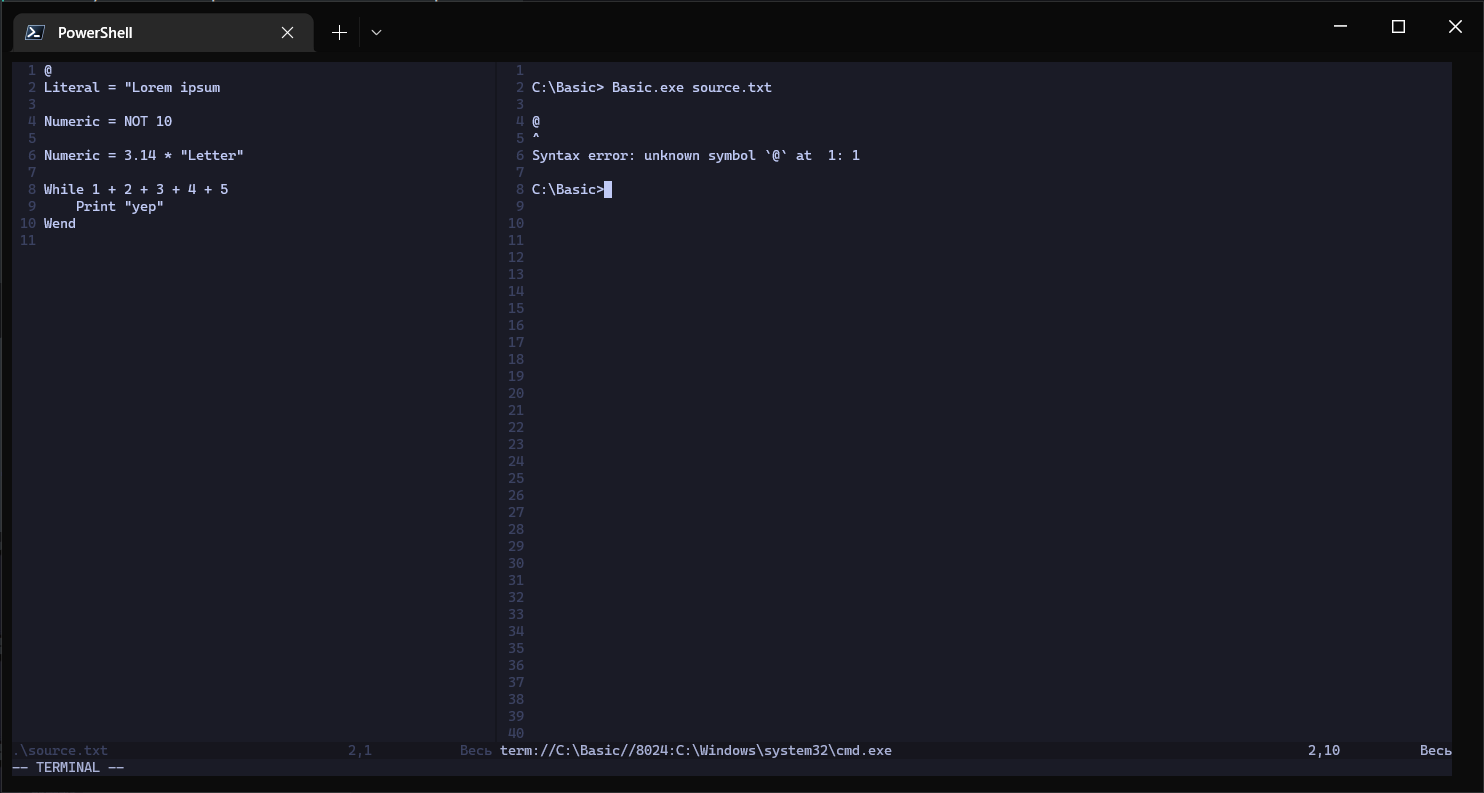
\includegraphics[scale=0.42]{image1.png}
    \caption{Синтаксическая ошибка 'неизвестный символ'}
    \label{error1}
\end{figure}

\begin{figure}[H]
    \centering
    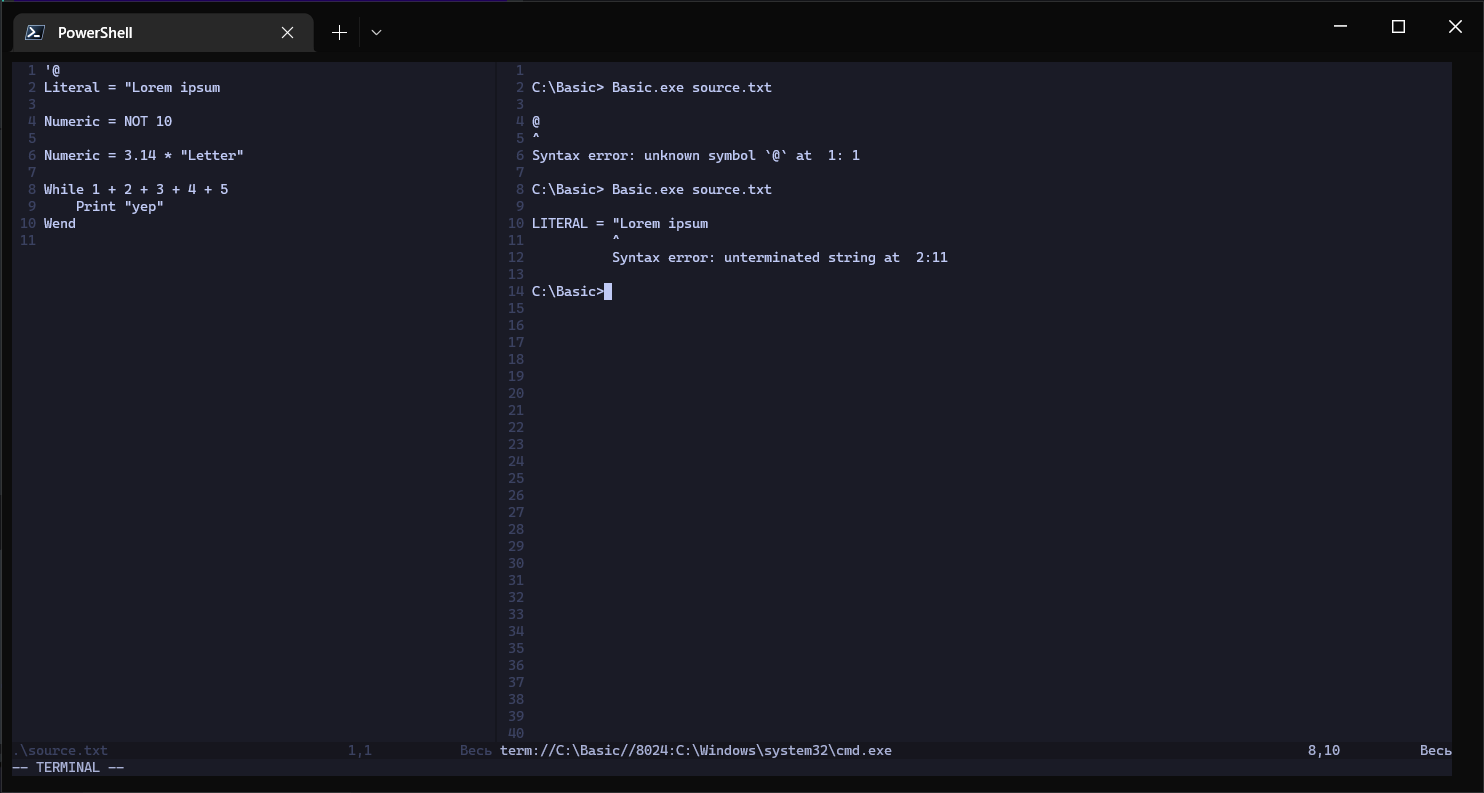
\includegraphics[scale=0.42]{image2.png}
    \caption{Синтаксическая ошибка 'незаконченная строка'}
    \label{error2}
\end{figure}

\begin{figure}[H]
    \centering
    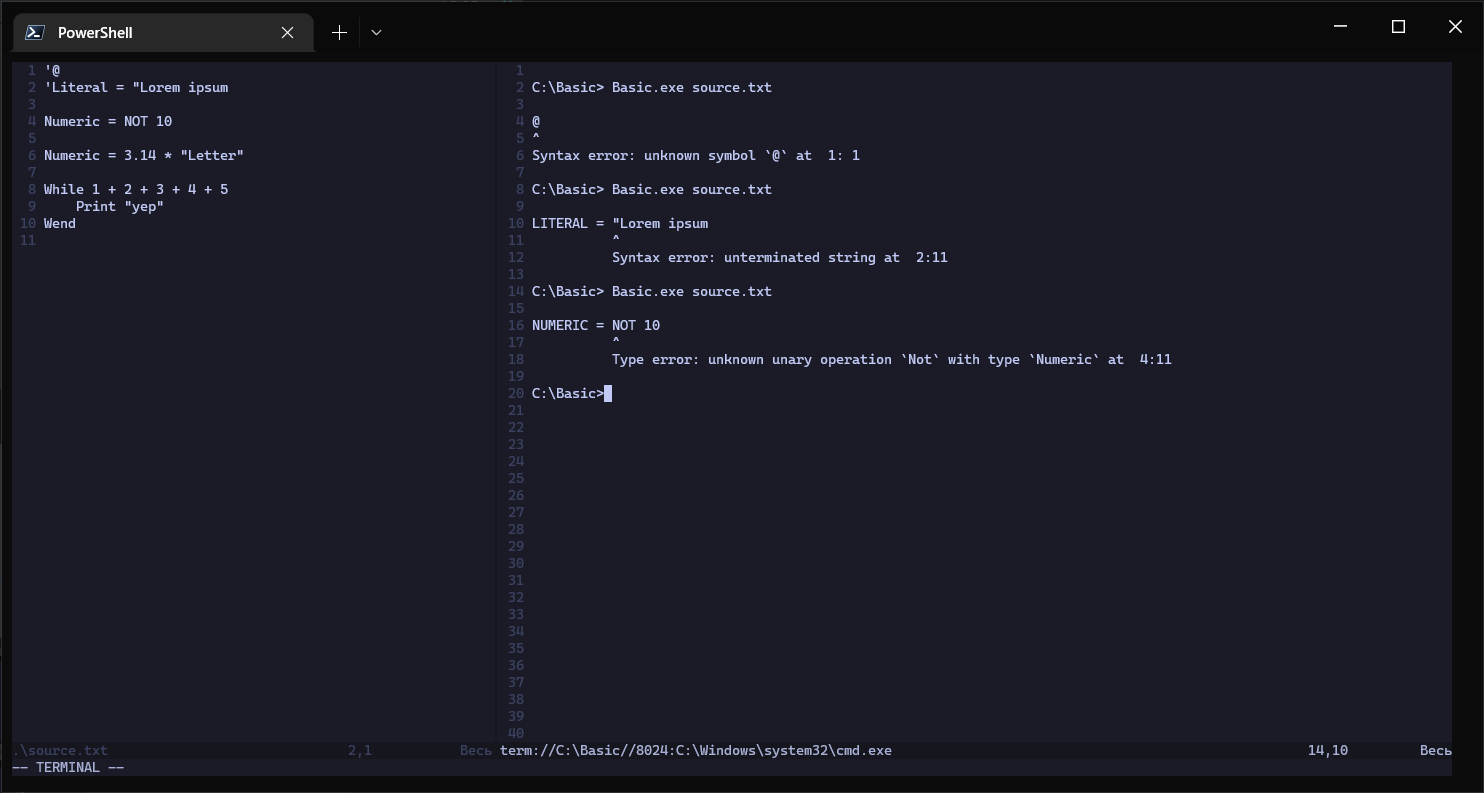
\includegraphics[scale=0.42]{image3.png}
    \caption{Синтаксическая ошибка 'неизвестная унарная операция'}
    \label{error3}
\end{figure}

\begin{figure}[H]
    \centering
    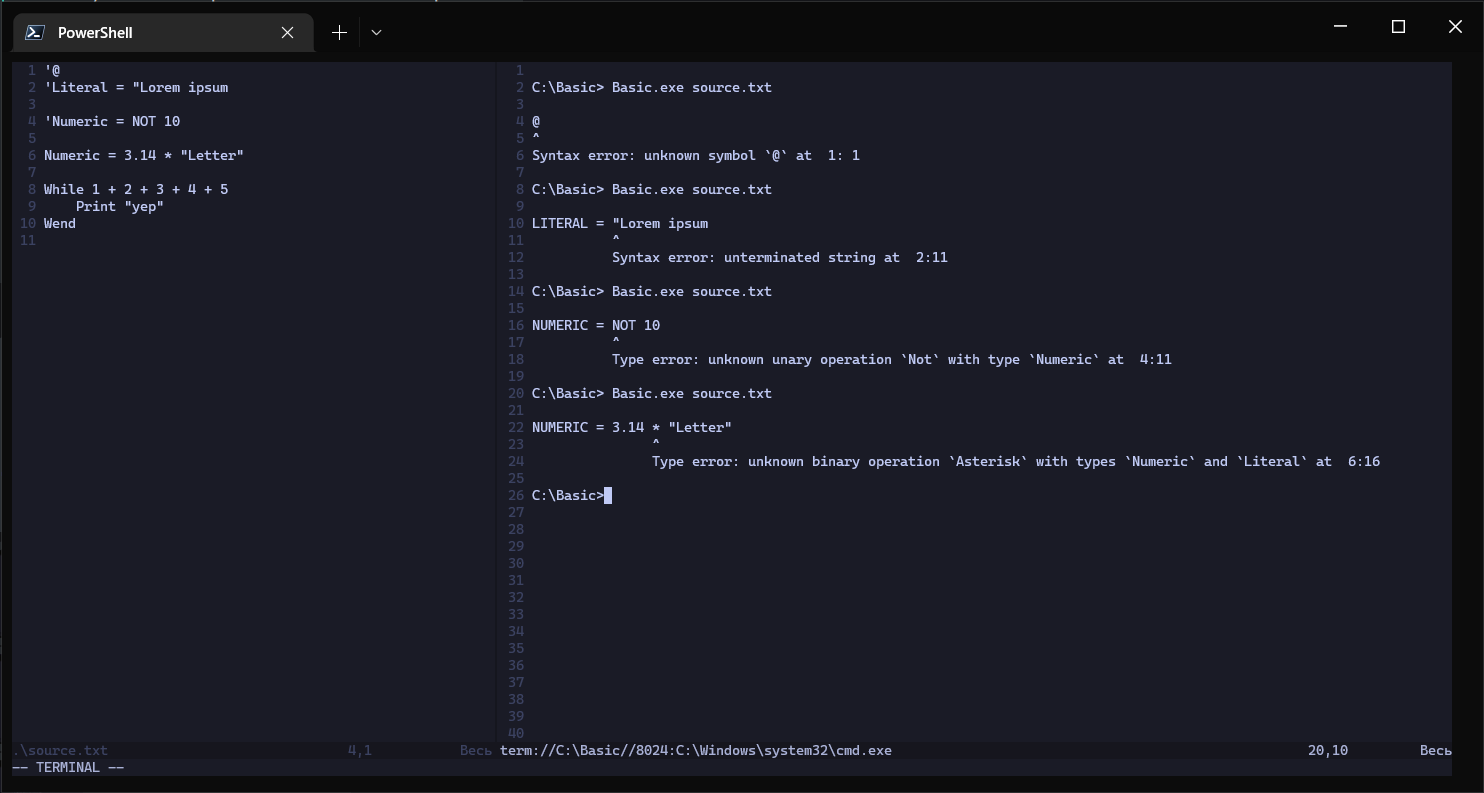
\includegraphics[scale=0.42]{image4.png}
    \caption{Синтаксическая ошибка 'неизвестная бинарная операция'}
    \label{error4}
\end{figure}

\begin{figure}[H]
    \centering
    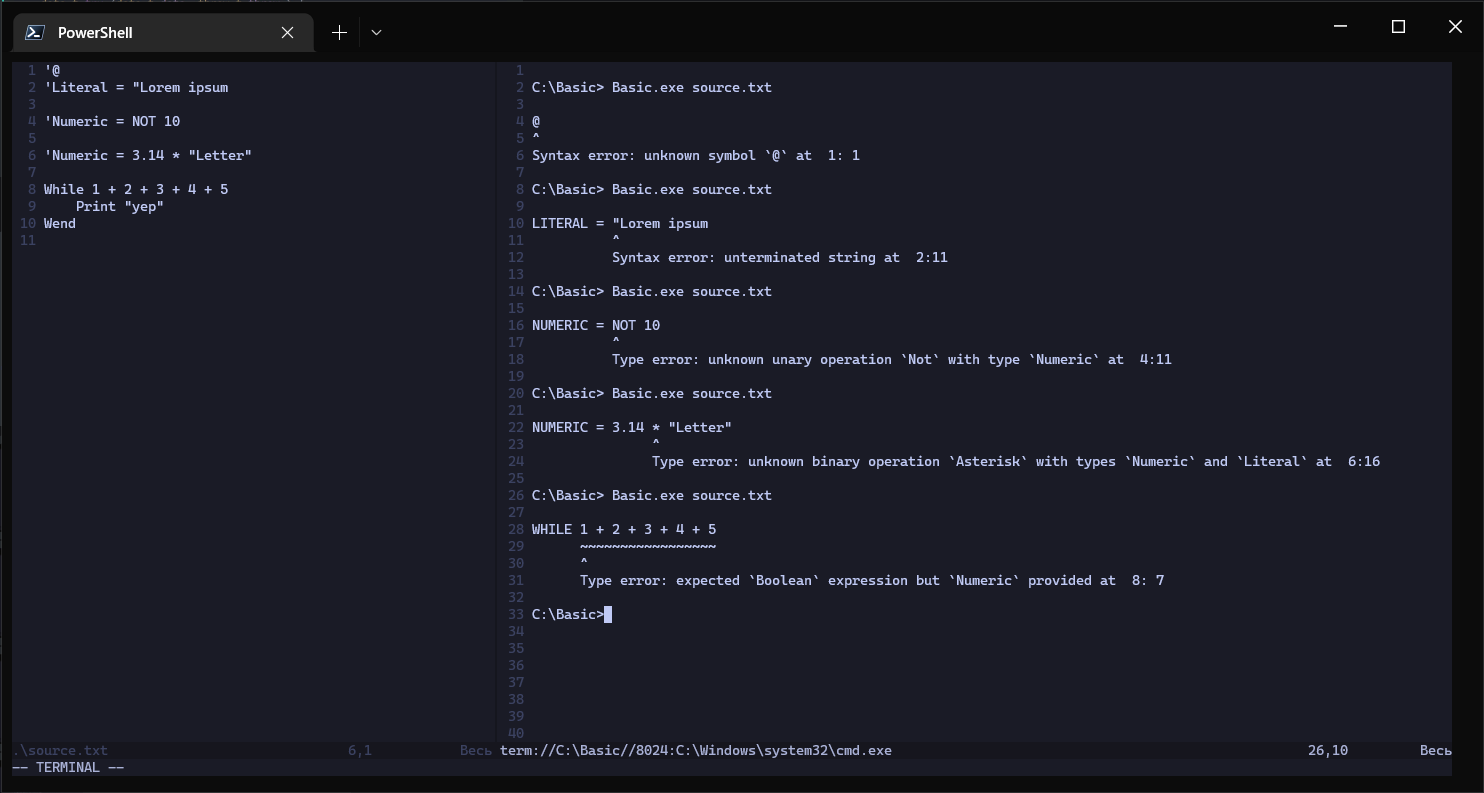
\includegraphics[scale=0.42]{image5.png}
    \caption{Синтаксическая ошибка 'неверный тип выражения'}
    \label{error5}
\end{figure}

\pagebreak

На рисунке \ref{guessing} изображен результат выполнения
программы, реализующей простую математическую игру <<Угадай число>>.

\begin{figure}[hb]
    \centering
    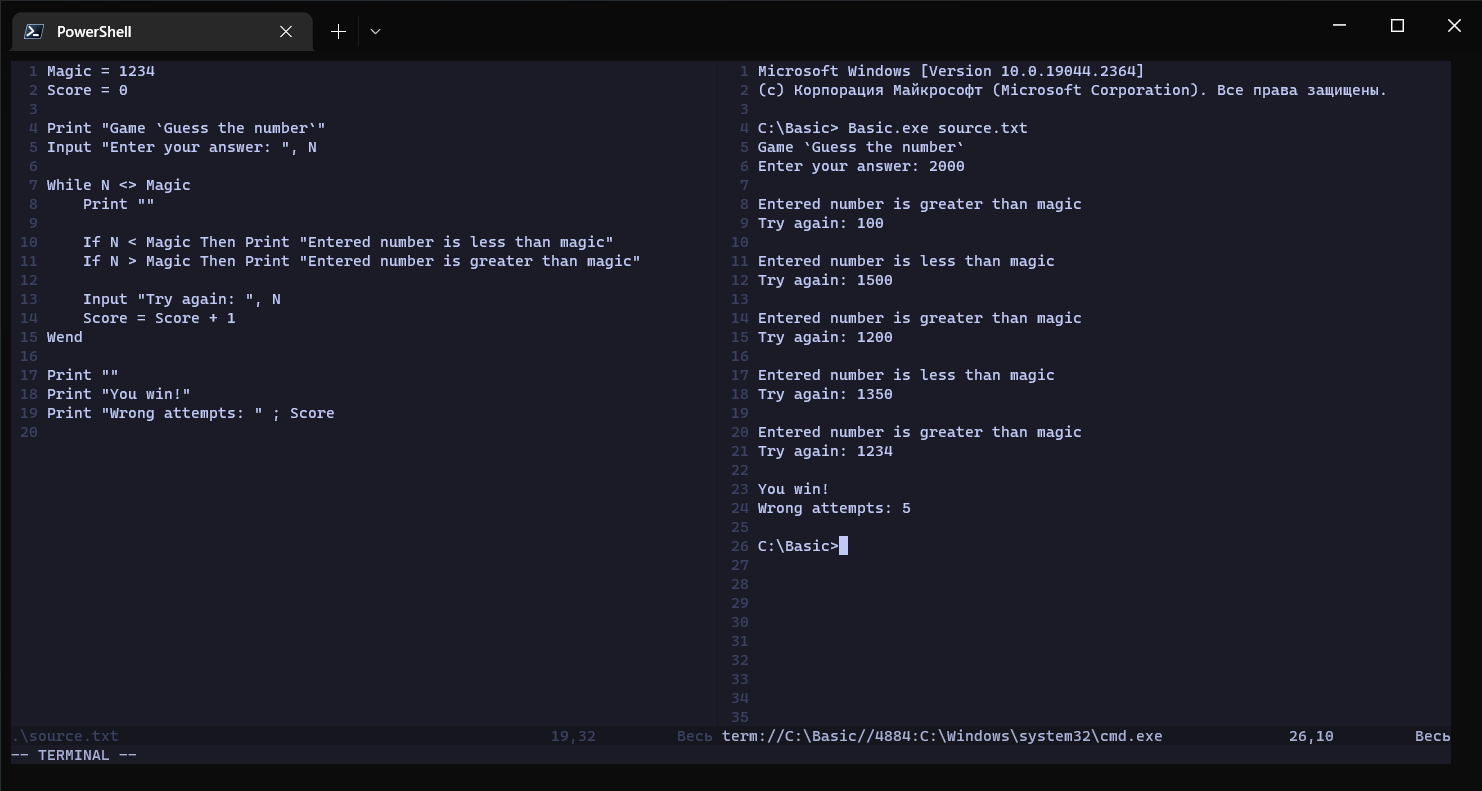
\includegraphics[scale=0.42]{image6.png}
    \caption{Результат успешного выполнения программы}
    \label{guessing}
\end{figure}       % Результат выполнения программы

    \csection{Заключение}

В данном разделе будут подведены итоги по проектированию осциллографа с интерфейсом к персональному компьютеру.

В ходе выполнения курсового проекта были получены теоретические сведения, необходимые для построения схем основных преобразований аналогового сигнала, таких как деление, умножение и смещение.
Примененные при разработке схемы электротехнические решения являются типовыми для современных осциллографов, что также способствует пониманию их внутреннего устройства.

Разработанный USB-осциллогаф имеет два канала с диапазоном входного сигнала
\begin{itemize}
    \item от -25 до 25 В при использовании щупов 1:1;
    \item от -250 до 250 В при использовании щупов 1:10.
\end{itemize}
и позволяет исследовать часто встречаемые в любительской среде аналоговые сигналы, например, аудиосигналы, ультразвук, переменный ток в лабораторных цепях, показания датчиков.

Полученная схема устройства имеет простую структуру, поэтому без проблем может быть усовершенствована, например, путем добавления логического анализатора для исследования дискретных сигналов, или наращиванием входного каскада для увеличения допустимого диапазона исследуемого аналогового сигнала.     % Заключение

    \renewcommand{\bibsection}{\csection{Cписок использованных источников}}

\phantomsection\pagebreak

\bibliography{bibliography}                     % Cписок использованных источников

    \appendix{обязательное}{Листинг программы}

\pagebreak
{\small\verbatiminput{resources/Source.txt}}       % Листинг программы
    \appendix{обязательное}{Диаграмма классов} \label{uml}

\includepdf[pages=1, fitpaper]{resources/UML.pdf}       % Диаграмма классов
    \appendix{обязательное}{Блок-схема алгоритма} \label{bss}

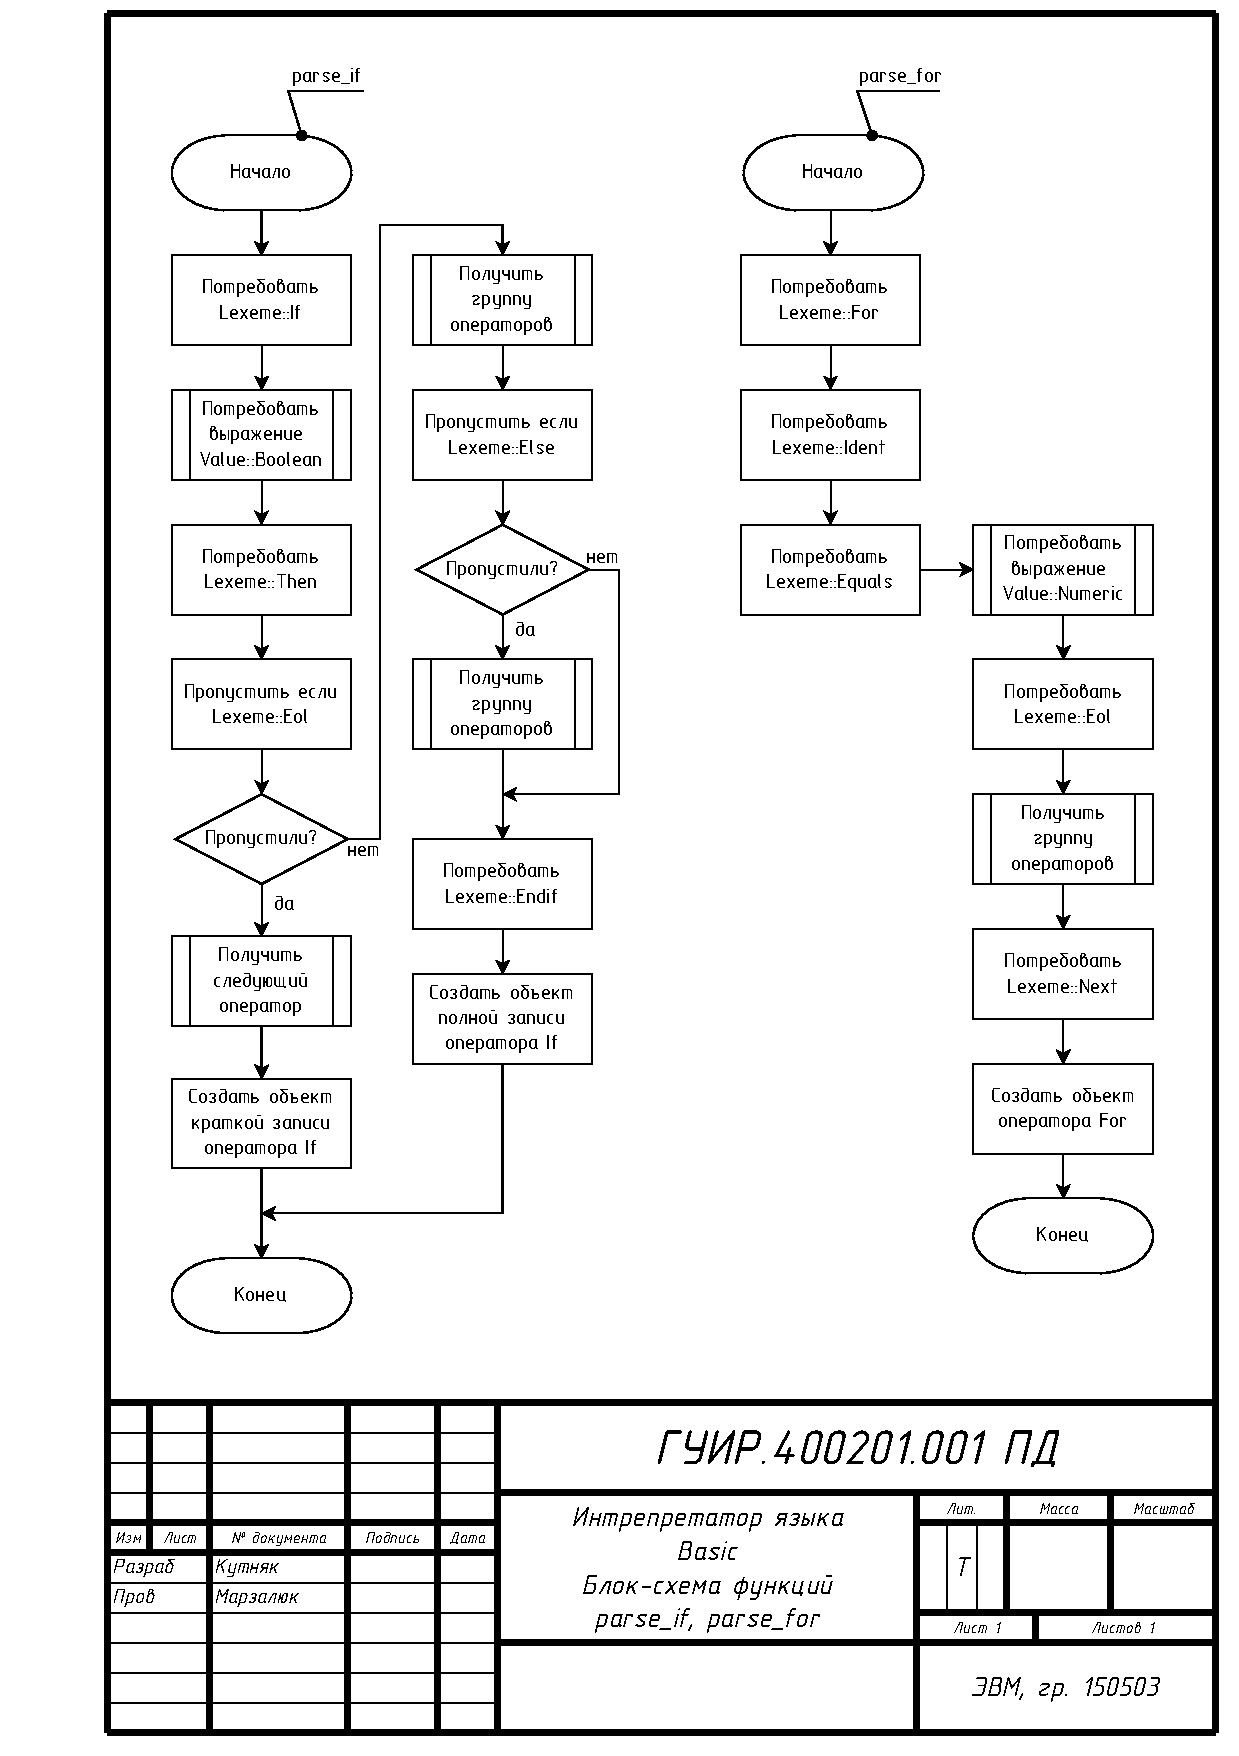
\includepdf{resources/Scheme.pdf}       % Блок-схемы алгоритмов
    \appendix{обязательное}{Ведомость документов}

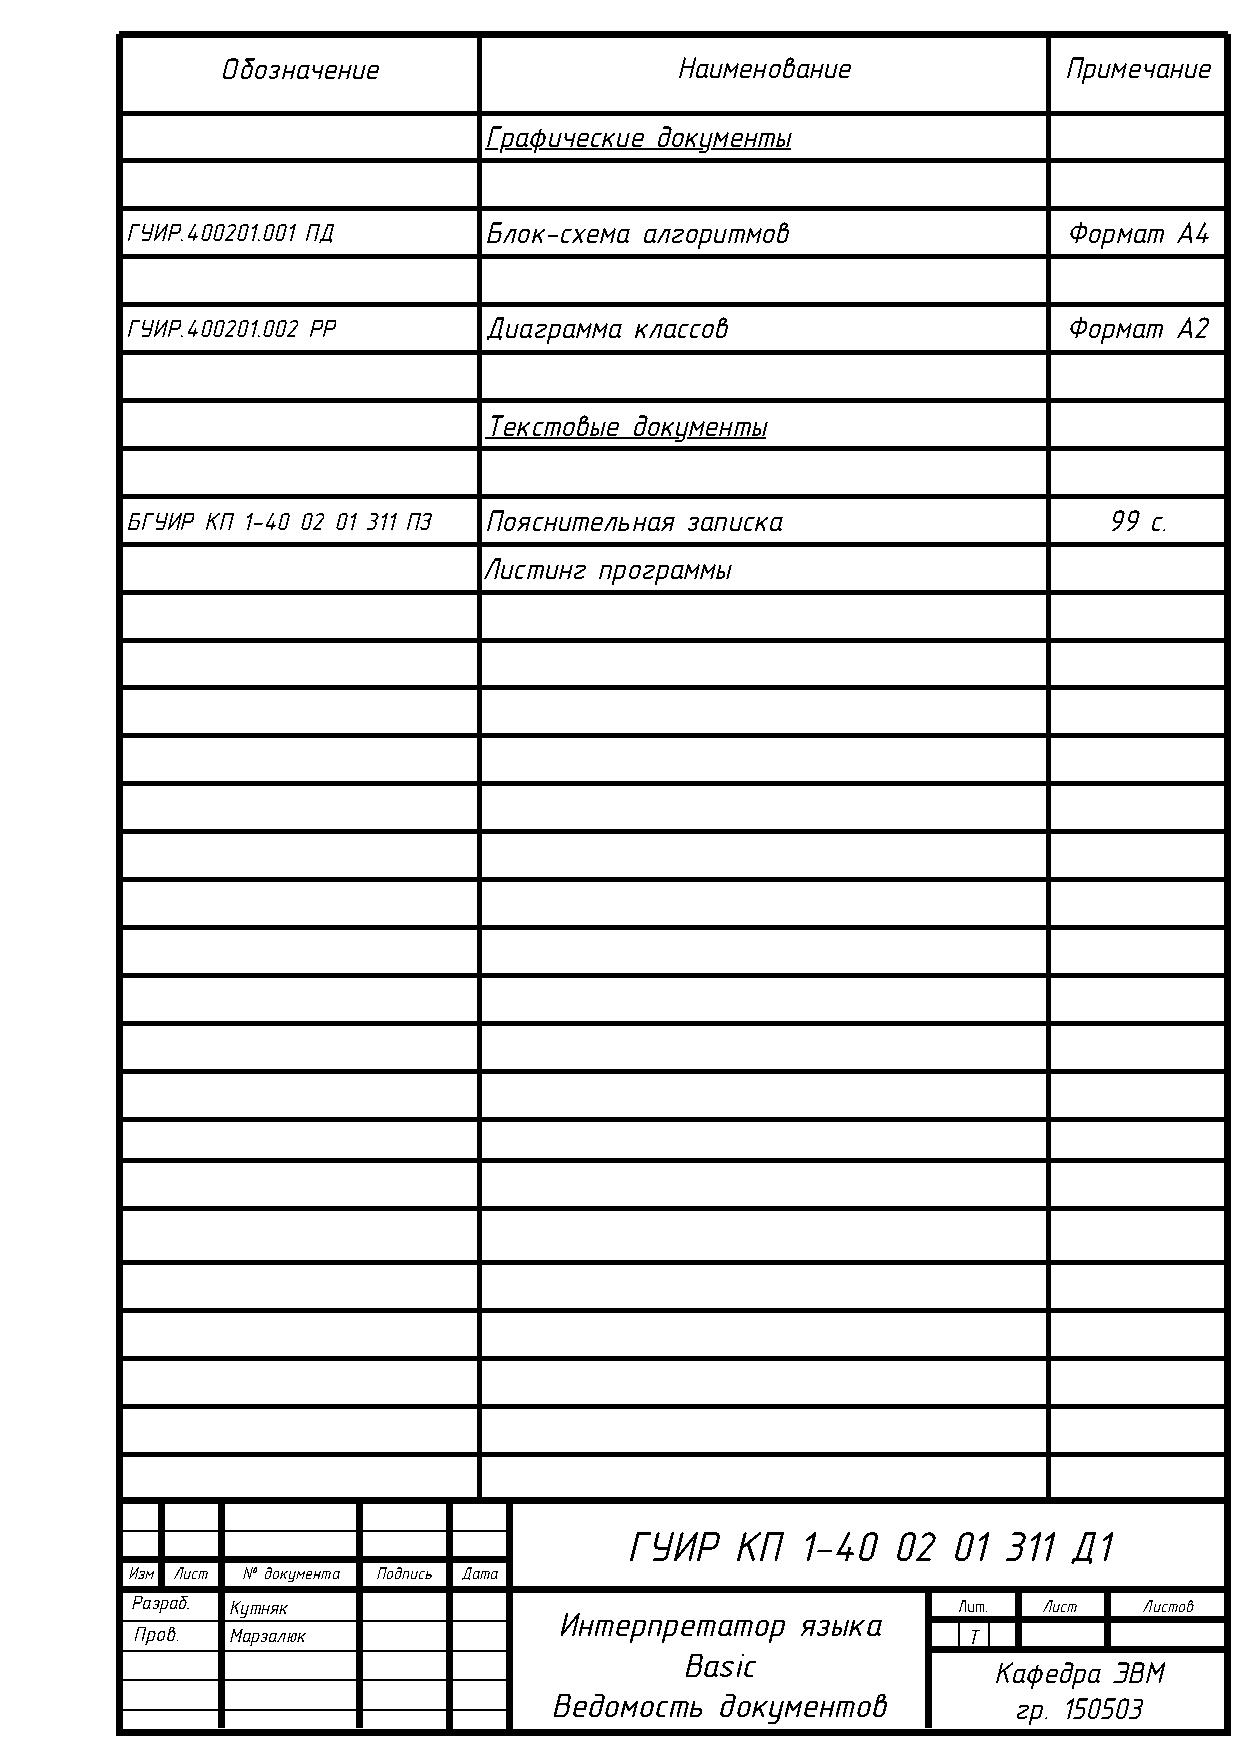
\includepdf{resources/Statement.pdf}       % Ведомость проекта

    \nocite{*}                          % Не искать цитаты

\end{document}